\chapter{Problem Definition}

\section{Description}

Given various aerial resources and fire fronts, a flight schedule needs to be created, such that the amount of water dropped by aerial resources approaches the target water content as much as possible in every discrete time slot and on every fire front, while at the same time adhering to numerous constraints~\cite{SkorinKapov/ILP}.
The duration of the schedule, exact capabilities of available aerial resources, the distribution of the target water content, etc., are input data for the problem.
In practice, they are determined by the incident commander, based on the current and expected future state of the wildfire, and his assessment.
The output is a complete flight schedule -- a list of all flights with their respective takeoff times and flight paths, i.e., fire fronts to which they are assigned.
It is created for a single day, which is often a part of a multi-day fire suppression effort.
Considering the incredible complexity and interaction of changing weather conditions, unpredictable spread of the fire, and uncertain impacts of suppression efforts, this schedule can only be considered as an estimate that will help in the planning phase of the entire operation.

A large-scale wildfire is often divided into two or more fire fronts (zones), which are handled separately.
During a single flight, an aircraft will work on a single fire front the entire time.
In case of smaller fires, aircraft tend to work in different areas of the fire during a flight as the fire is being extinguished.
However, we focus on large-scale wildfires, where it is common practice for aerial resources to spend a single flight fighting the fire in the same general area, while also maximizing the allowed flight duration.
Each fire front commonly has one or more dedicated water points where aircraft can refill their water tanks, which is predetermined and not a part of the schedule.

Two types of aerial resources are considered: fixed-wing aircraft and rotary-wing aircraft.
Fixed-wing aircraft are referred to simply as \textit{airplanes}, and sometimes as airtankers, water bombers, or amphibious airplanes.
Rotary-wing aircraft are simply called \textit{helicopters}.
A photograph of a fixed-wing aircraft making a drop of water is shown in Figure~\ref{fig:canadair-drop}.

\begin{figure}[tb]
    \centering
    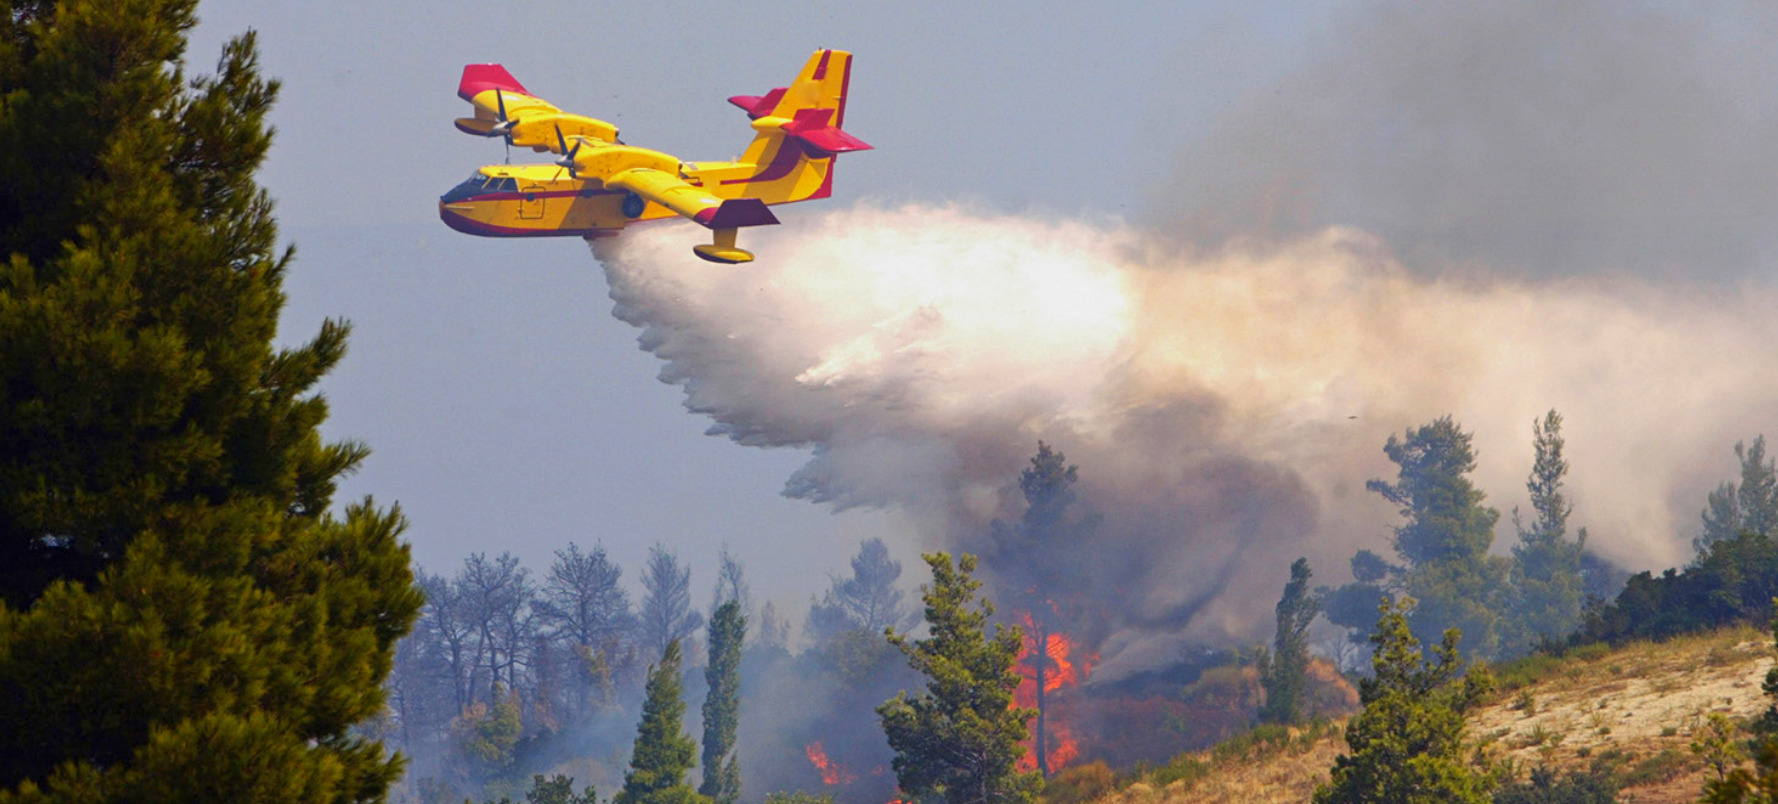
\includegraphics[width=0.95\linewidth]{img/canadair-drop.jpg}
    \caption{An amphibious aircraft dropping water on a wildfire~\cite{Viking/CL415Sheet}}
    \label{fig:canadair-drop}
\end{figure}

In order to model the scheduling problem, we divide the daylight hours into discrete time slots of fixed duration.
Twenty minute increments are selected, because in practice almost every relevant duration is a multiple of 20 minutes.
However, the duration can be easily changed if needed.
In fact, it is implicit -- everything is measured in terms of time slots, and not minutes or hours.

Because time is expressed in discrete time slots, instead of any real value, all decision variables are discrete, too.
The search space is a finite, albeit enormous, set of feasible discrete schedules, and the goal is to find the best one.
Therefore, the task at hand is an NP-hard combinatorial optimization problem.

Once an aircraft arrives at the fire front, it will most likely make multiple drops of water before returning to base.
To do that, it must refill in flight, including before arrival.
Because of their characteristics, helicopters and airplanes refill differently, and have different flight paths and flight speed.
Airplanes refill by scooping from a sufficiently long body of water, shown in Figure~\ref{fig:scooping}, whereas helicopters are often equipped with a bucket which they lower into the water while hovering at a low altitude.
If both types of aircraft were present at the same fire front, airspace coordination would become much more demanding, increasing the odds of an accidental collision.
Therefore, only one type of aircraft may operate at a fire front at the same time.

\begin{figure}[htb]
    \centering
    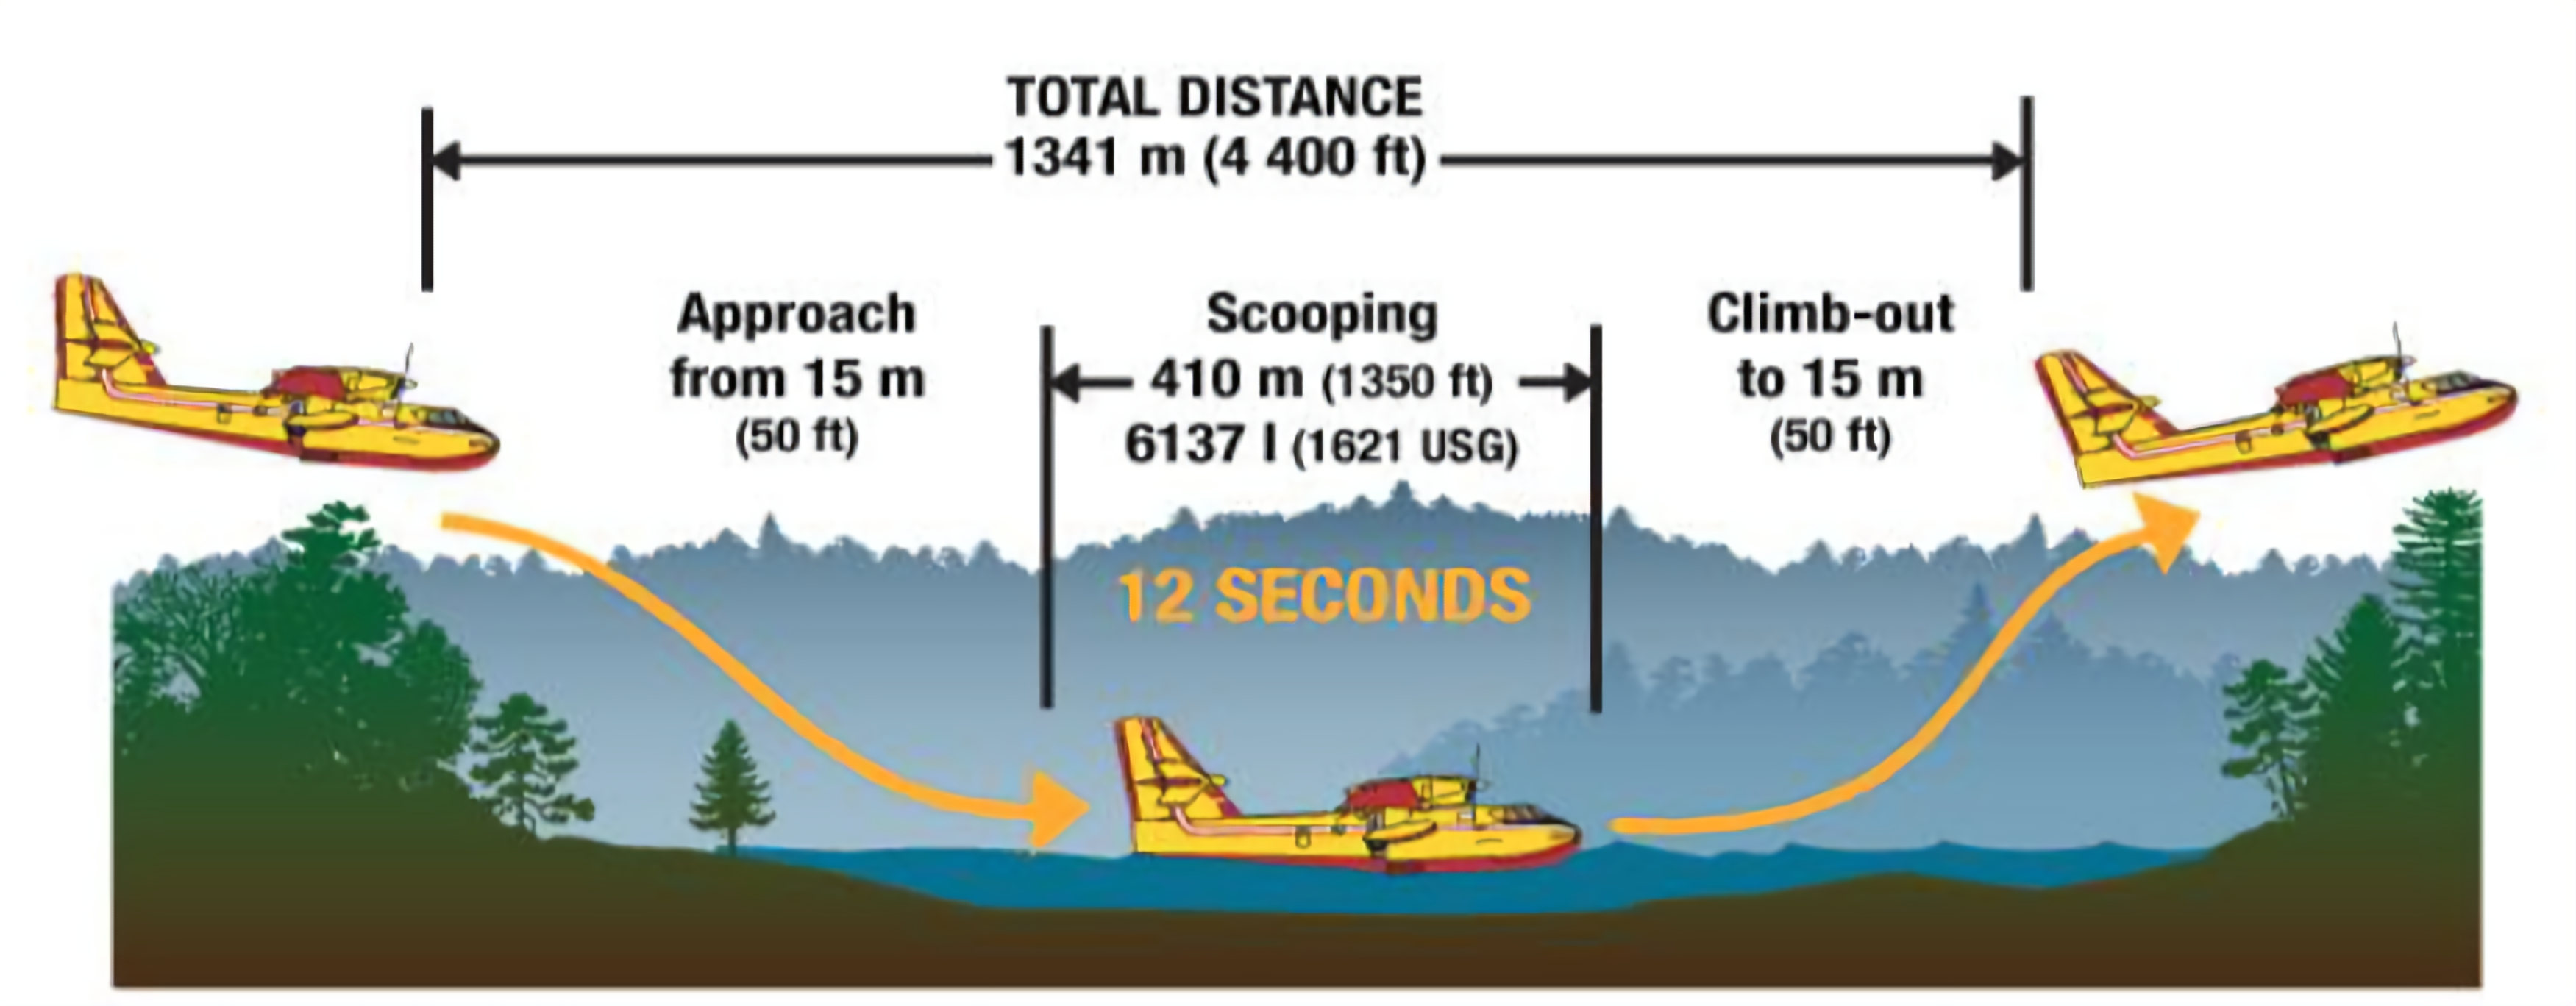
\includegraphics[width=0.95\linewidth]{img/scooping.jpg}
    \caption{An illustration of water scooping by an amphibious aircraft~\cite{Viking/Technique}}
    \label{fig:scooping}
\end{figure}

Helicopters can refill from a small body of water (e.g., a narrow river, a small lake, swimming pools, etc.), whereas airplanes cannot.
If a fire front has only such smaller water points in its vicinity, airplanes will have very limited usability as they will have to make long flights in order to refill at a further, larger water point.
Additionally, if the terrain is generally particularly difficult, it might be inaccessible to airplanes.
Consequently, some fire fronts have restrictions which allow only helicopters to be assigned to those fronts.

When multiple aerial resources are active at the same fire front at the same time, they fly in a carousel-like formation,\footnote{Simply referred to as a \textit{carousel}.} meaning that they are on a very similar flight route, following one another.
The flight route is a circular path defined by the water refilling point, and the discharge point.
An example of a flight route is shown in Figure~\ref{fig:carousel}.
To avoid overcrowding the air space, a limit is set on the number of aerial resources that can fly at the same time at the same front, depending on the fire front.
The limit can depend on the size of the fire front, and the distance and size of the water point.

\begin{figure}[htb]
    \centering
    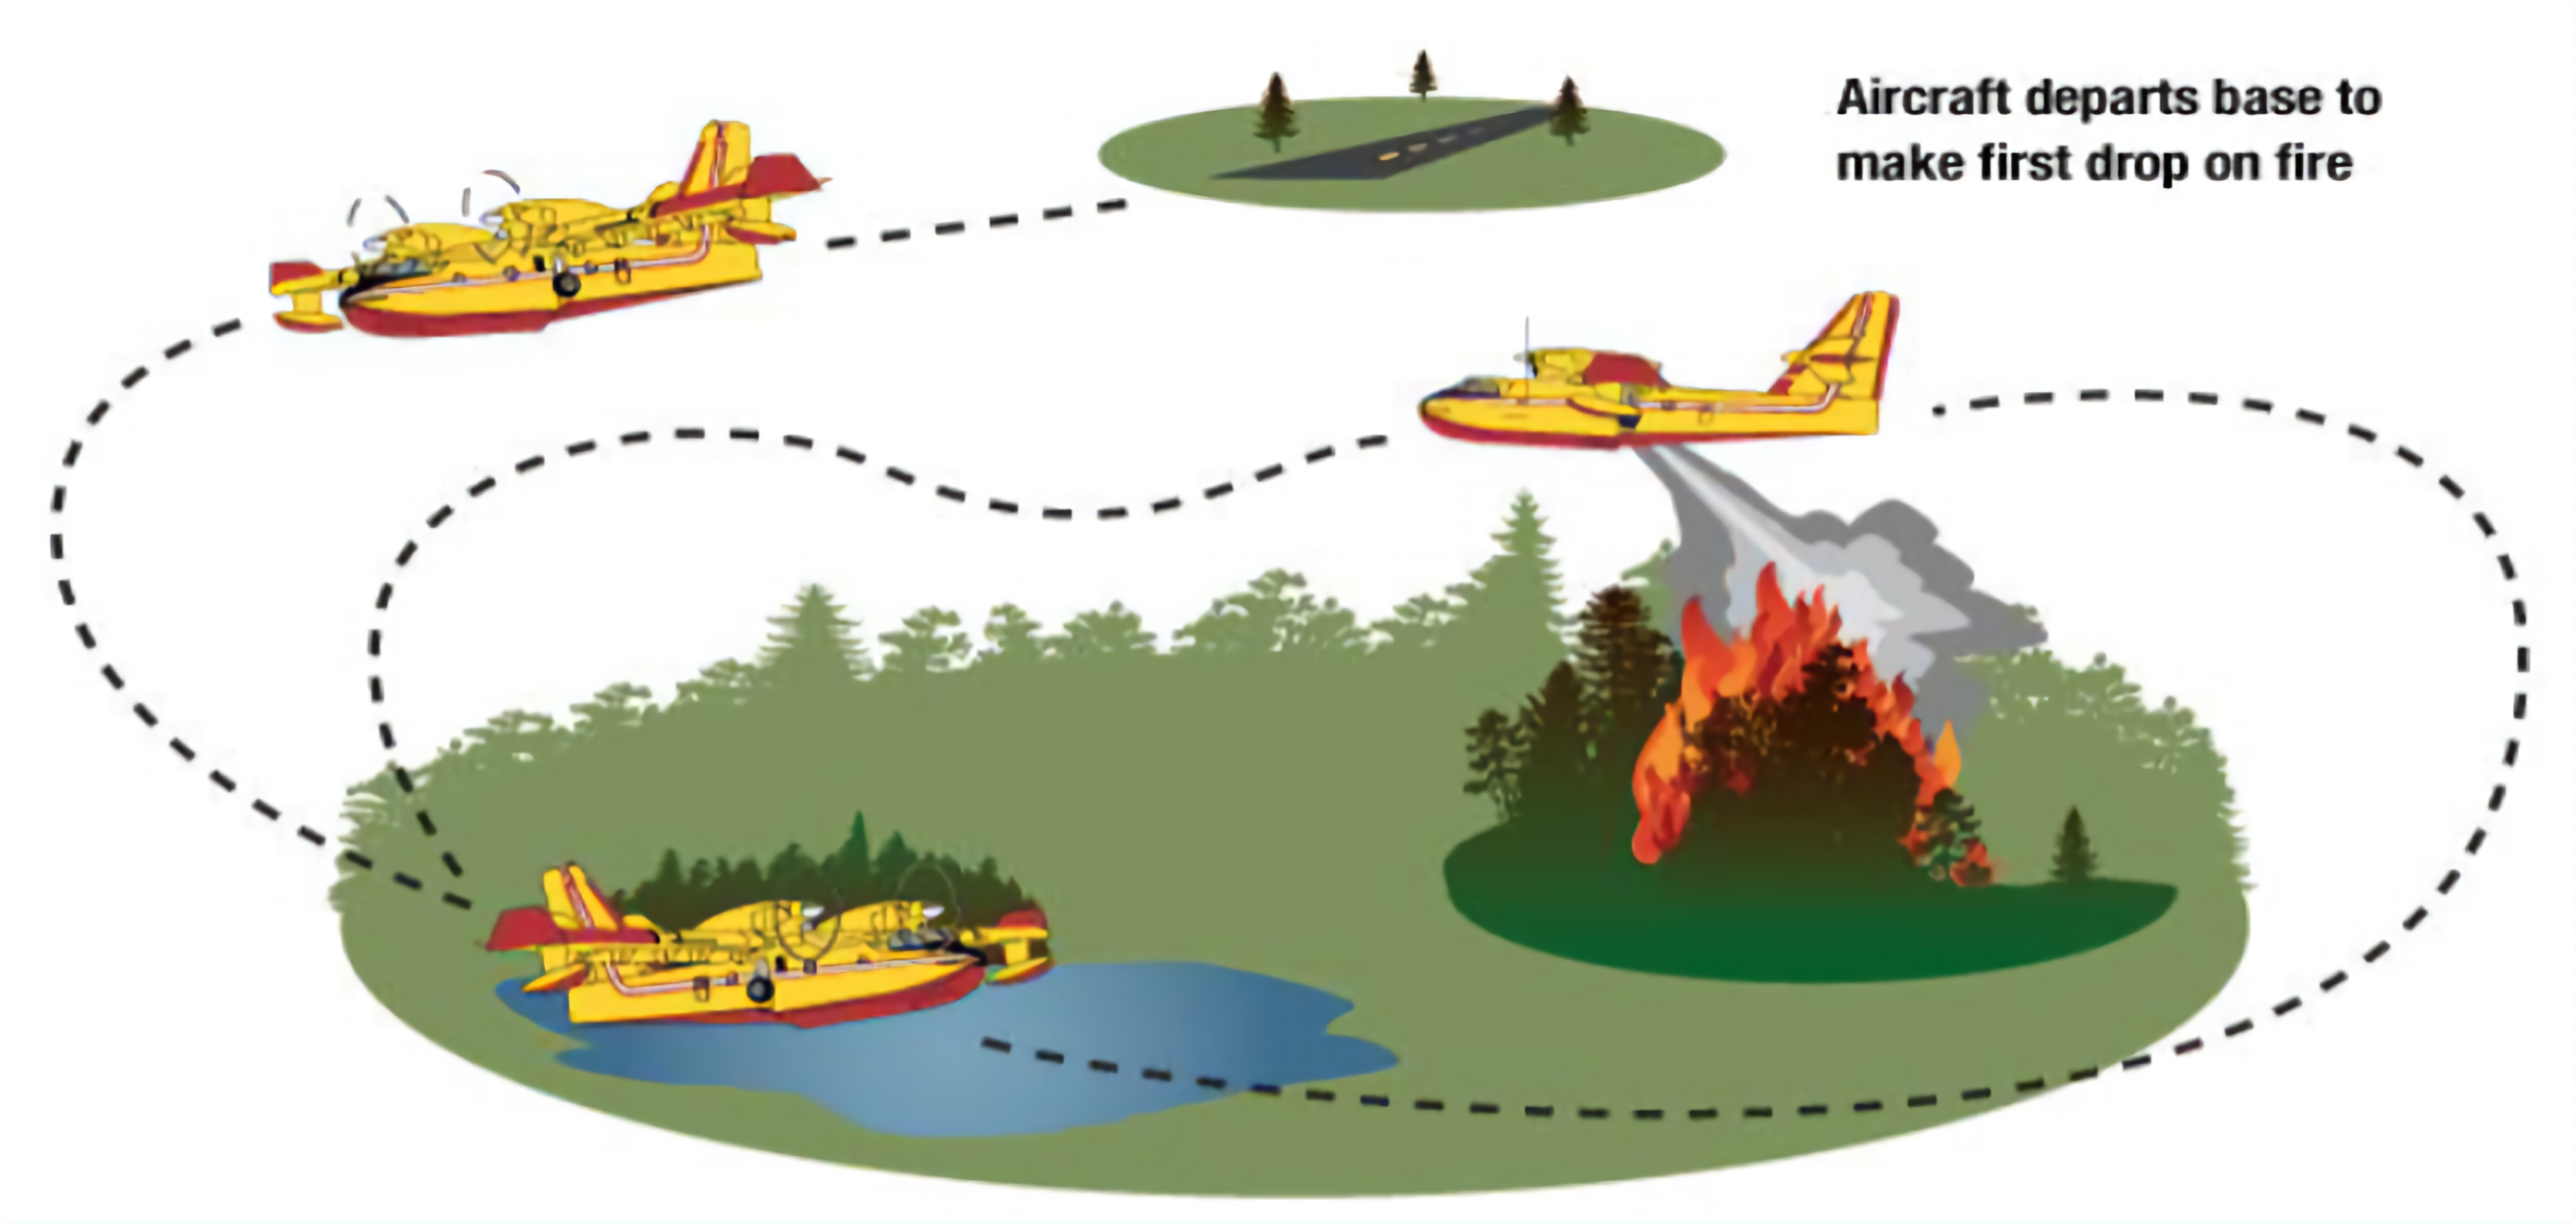
\includegraphics[width=0.95\linewidth]{img/carousel.jpg}
    \caption{A flight path which includes takeoff and repeated filling and dropping of water~\cite{Viking/Technique}}
    \label{fig:carousel}
\end{figure}

Creating a flight schedule cannot be done without taking the pilots (and the rest of the crew) into consideration.
In practice, one flight crew is assigned to one aircraft during a single day, and vice versa.
For that reason there is no need to differentiate between pilots and resources in this model, and whichever rules apply to the crew, also apply to the aircraft.
The terms \textit{aircraft}, \textit{pilot}, and \textit{flight crew} are used interchangeably, with the first being the most common.

Under Spanish regulation, a crew member must not be active for more than 12 consecutive hours~\cite{Spain/AnnexCircular}.
In a special case where the crew consists of military personnel, the 12 hour limit can be extended if resting periods are prolonged.

Between two consecutive flights, the crew must rest and the aircraft must be refueled.
The aircraft is inspected and, if needed, minor repairs can be made during this time.
In this model, we assume all resources will be working properly during availability time slots.
A minimum resting period is prescribed, depending on the duration of the previous flight, and the aircraft type.

Aerial resources are not necessarily available during the entire day.
Airplanes are deployed relatively sparsely, as shown in Figure~\ref{fig:spain-airplanes-deployment}.
On the other hand, helicopters are often readily available in the proximity of the fire, as they require less infrastructure and are overall more common.
In case an airplane was stationed in a faraway base prior to arriving to the general area of the wildfire, it is considered unavailable during the transit.
The same applies when the airplane is returning to another base at the end of the day.
Once the airplane reaches the general area of the wildfire, it is usually stationed in a relatively close base for several days, from where it engages the wildfire.
It is assumed that the mandatory resting period after the transit flight is included in the unavailability period.

Aerial firefighting in itself is significantly more dangerous than flying in normal conditions.
It requires performing special high-risk maneuvers, such as refilling water tanks mid-flight, flying at a low altitude, navigating difficult terrain, or avoiding vertical obstructions like power lines and wind turbines.
Exacerbating factors also include stronger winds, increased temperature, and reduced visibility due to the thick smoke, all caused by the large wildfire.
If we were to add night-time into the equation, the flight would become even more difficult and the risk of an accident would significantly increase.
Therefore, regulations dictate that aerial resources are not permitted to fight fires during night-time hours~\cite{Spain/AnnexCircular}, and the flight schedule is to be created only for the daytime.
While it could be possible for aircraft to perform longer transits at night-time, be it early in the morning or late in the evening, effectively extending the flight schedule, it is not considered in this model.


\section{Phases of Flight}

In each 20-minute time slot, an aerial resource may be active or inactive.
Active resources may be in one of three states:
\begin{itemize}
    \item \textbf{Transit:} travelling to or from the fire front during the entire time slot,
    \item \textbf{Hybrid:} arriving or departing from the fire front during the time slot. The resource spends some time in transit, and some time fighting the fire.
    \item \textbf{Firefighting:} actively fighting the fire during the entire time slot.
\end{itemize}

Consider a flight of duration $T \in \mathbb{N}$ with $u \in \mathbb{N}_0$ transit slots in each direction.
Let the flight begin in time slot $t$.
The previously discussed states correspond to the following time slots (also depicted in Figure~\ref{fig:phases-flight}):
\begin{itemize}
    \item Departing transit time slots: $[ t,\ t + u \rangle$,
    \item First hybrid time slot (arrival at fire): $t + u$,
    \item Firefighting time slots: $[ t + u + 1,\ t + T - u - 1 \rangle$,
    \item Second hybrid time slot (departure from fire): $t + T - u - 1$,
    \item Returning transit time slots: $[t + T - u,\ t + T \rangle$.
\end{itemize}

\begin{table}[htb]
\vspace{0.8\baselineskip}
\centering
\fontsize{9.5pt}{10pt}\selectfont
\begin{tabular}{@{}*5c@{}}
$t~~\cdots~~t+u-1$ & $t+u$ & $t+u+1~~\cdots~~t+T-u-2$ & $t+T-u-1$ & $t+T-u~~~\cdots~~~t+T-1$ \\
\upbracefill & \upbracefill & \upbracefill & \upbracefill & \upbracefill \\
Transit & Hybrid & Firefighting & Hybrid & Transit \\
\end{tabular}
% Faking a Figure, as the illustration is not really a proper table.
\captionof{figure}{Time slot ranges corresponding to different phases of flight} \label{fig:phases-flight}
\end{table}

Some groups of time slots may be empty, depending on parameter values.
If an aircraft is stationed close to a fire front, it is likely that there will be no transit slots, as the aircraft can reach the front within a single time slot.
Helicopters can be stationed at a variety of locations and tend to be within 20 minutes of flight time from the fire~\cite{INFOCACongreso2017}.
Airplanes are required to be stationed at airbases or airports, and typically have longer transit times (e.g., 40 minutes). 
On the other hand, due to the long transit times to and from a distant fire front, it is also technically possible for a flight to have no firefighting time slots.
Such flights are a poor use of available resources, but are not forbidden.
In the exceptional case that the aircraft barely reaches the fire front and already has to start returning to the base in the same time slot, it would be even less efficient than in a regular hybrid time slot.
However, such hybrid slots are not considered in this model, and are treated as if they were a regular hybrid slot.

Aircraft's suppression potential is measured in terms of the number of drops per time slot and fire front.
Note, the number of drops will differ between fronts due to locations of refill points.
Furthermore, they can differ over time due to meteorological conditions affecting flights and refill constraints.
For example, stronger winds may force an aircraft to fly slower, or take a different, longer flight path.
The number of drops is given as a real number, and not an integer, because it represents an estimated average value.
For example, if the value is $1.5$ drops per time slot, the aircraft will likely make one drop in one time slot, and two drops in the other time slot.
The amount of water dropped per time slot is calculated by multiplying the water capacity of the aircraft, with the estimated number of drops per time slot.
All values are given as problem input parameters.

When an aircraft is in a hybrid time slot, it spends some time traveling from the base.
To represent the amount of time spent in transit in such time slots, which depends on the distance from the base to the fire and the current weather conditions, the number of drops per time slot is proportionally smaller compared to a firefighting time slot.


\section{Parameters}

\subsection{Input Parameters}

All problem input parameters, their types and descriptions are listed in Table~\ref{tbl:input-params}.

\begin{table}[htb]
\caption{Descriptions and types of problem input parameters}
\label{tbl:input-params}
\small
\centering
\begin{tabularx}{\hsize}{@{}llX@{}}
Parameter & Type & Description \\
\midrule
$k,\ \mathcal{K}$ & -              & Index and set of aerial resources. \\
$f,\ \mathcal{F}$ & -              & Index and set of fire fronts. \\
$t,\ \mathcal{T}$ & -              & Index and set of consecutive time slots. \\
$V_k$             & $\{0,1\}$      & $1$ if aircraft $k$ is a helicopter, $0$ if it is an airplane. \\
$T_k$             & $\mathbb{N}$   & The flight duration of aircraft $k$, measured in time slots. \\
$R_k$             & $\mathbb{N}$   & The minimum resting period for aircraft $k$, measured in time slots. \\
$N_k$             & $\mathbb{N}$   & The maximum number of flights aircraft $k$ can perform in one day. \\
$P_k$             & $\mathbb{N}$   & The maximum number of continuous time slots in which a pilot is active, including flying and resting time. \\
$A_k^t$           & $\{0,1\}$      & $1$ if aircraft $k$ is available in time slot $t$, $0$ if it is not. \\
$B_{f}$           & $\{0,1\}$      & $1$ if only helicopters can fly on front $f$, $0$ if all types of aircraft can fly on that front. \\
$U_{kf}$          & $\mathbb{N}_0$ & The number of full time slots needed for aircraft $k$ to reach the front $f$. \\
$W_f^t$           & $\mathbb{R}^+$ & The target water content for fire front $f$ in time slot $t$, measured in liters. \\
$S_f$             & $\mathbb{N}$   & The maximum number of resources which can fly at front $f$ at one time. \\
$C_k$             & $\mathbb{N}$   & The water capacity of aircraft $k$, measured in liters. \\
$D_{kf}^t$        & $\mathbb{R}^+$ & The average number of drops aircraft $k$ will make over fire front $f$ in time slot $t$ if it spends the entire time slot actively fighting the fire. \\
$E_{kf}^t$        & $\mathbb{R}^+$ & The average number of drops aircraft $k$ will make over fire front $f$ in time slot $t$ if it is arriving to or leaving the fire front in that time slot. \\
$a_1, a_2, a_3$   & $\mathbb{R}^+$ & The weighting factors used in the objective function (see Section~\ref{sec:objective}). \\
\end{tabularx}
\end{table}


\subsection{Decision Variables}

The flight schedule is unambiguously determined by a takeoff matrix with elements \hbox{$c_{kf}^t \in \left\{ 0, 1 \right\}$}.
If the aircraft $k$ is initiating a flight towards the fire front $f$ in the time slot $t$, the element $c_{kf}^t$ will have value $1$.
Otherwise, the value of $c_{kf}^t$ will be $0$.

Because each aircraft's flights have a predetermined duration $T_k$, the state of each aircraft is known in every time slot solely based on the values of the takeoff matrix.
Consequently, the takeoff matrix is the only necessary decision variable for determining the flight schedule.


\subsection{Auxiliary Variables}

Water surplus in time slot $t$ on fire front $f$ is denoted by the variable $\mathit{WS}_{tf}$.
Water surplus is the difference between the amount of water that was dropped by all resources on that front in that time slot, and the target water content for that time slot and fire front.
If the value is negative, it means that particular target water content was not satisfied.
A positive value indicates that a larger amount of water was dropped than necessary, which is beneficial.

The sum of all water surplus values which are negative is called the negative water surplus, denoted by $\mathit{WS}_n$, and defined in Equation~\ref{eq:wsn-def}.
$\mathit{WS}_n \le 0$ always holds.
\begin{equation}\label{eq:wsn-def}
\mathit{WS}_n = \sum_{t \in \mathcal{T}} \sum_{f \in \mathcal{F}} \min (\!\mathit{WS}_{tf}, 0 )
\end{equation}

The minimal water surplus $Z$ is the smallest water surplus value, defined in Equation~\ref{eq:z-def}.
It may have any real value, but Equation~\ref{eq:z-wsn-relation} always holds.
\begin{equation}\label{eq:z-def}
Z = \min_{\substack{t \in \mathcal{T}\\f \in \mathcal{F}}} \mathit{WS}_{tf}
\end{equation}
\begin{equation}\label{eq:z-wsn-relation}
\mathit{WS}_n = 0 \iff Z \ge 0
\end{equation}

The total water output $\mathit{WO}$ is calculated as the sum of the amount of dropped water over all fire fronts and time slots.
This value is equal to zero if and only if the flight schedule is empty.
Otherwise, the total water output is a positive value.


\section{Objective Function}\label{sec:objective}

The objective function in Equation~\ref{eq:objective} maximizes the weighted sum of three distinct terms, representing three objectives of varying importance, regulated by weighting factors $a_1$, $a_2$, and $a_3$, in that order.
The first term is the sum of negative water surplus over all fire fronts and time slots, which is always negative or equal to zero.
The second term is the minimal water surplus over all fronts and time slots, which may have any real value.
Finally, the third factor is the total water output across all fronts and time slots, which is always non-negative.

\begin{equation}\label{eq:objective}
\max \left( a_1 \cdot \mathit{WS}_n
    + a_2 \cdot Z
    + a_3 \cdot \mathit{WO} \right)
\end{equation}

The original intention was to use the target water content as a hard constraint, meaning any flight schedule which did not meet all targets was unacceptable.
In that scenario, the water surplus would be positive across all fronts and time slots:
\begin{equation}
\mathit{WS}_{tf} \ge 0,\ \forall t \in \mathcal{T},\ \forall f \in \mathcal{F}
\end{equation}
Consequently, the first objective would always be equal to zero for feasible schedules.
Additionally, the second objective would always be positive, meaning the value of the entire objective function would also be positive.

However, meeting the target water content may not be possible, as will be described in detail in Section~\ref{sec:water-distribution}.
In order to solve that issue, meeting the target water content was changed to be a soft constraint, and the concept of maximizing negative water surplus was introduced into the objective function, as shown in Equation~\ref{eq:objective}.
That way schedules which do not meet the targets are penalized, but still considered feasible.

The second term in the objective function is used to facilitate spreading the water surplus more evenly across all time slots and fire fronts.
While other measurements, such as variance of water surplus, could achieve that goal more effectively, using a minimum value keeps the objective function, as well as the entire problem, linear.
It also keeps the model as similar as possible to the one in Ref~\cite{SkorinKapov/ILP}, which is needed for later comparisons of results.

The third term should be considered the least important of the three objectives.
While the total water output is a good measure of how effectively the resources were used in terms of their raw output, it is not indicative of the quality of the suppression efforts.
Dropping a large amount of water on some fronts or time slots, while leaving others neglected, can seriously harm the overall fire suppression.
It is much more beneficial to output less water overall, but in a more uniform manner, especially if the target water content was not met.
That being said, even if some flight does not impact the first or second term, it is still beneficial to schedule it and output more water in total.

Depending on the values of the weights $a_1$, $a_2$, and $a_3$, if the value of the objective function is positive, it is not indicative of the fact that all water content targets have been satisfied.
However, if the value of the objective function is negative, it is certain that the targets have not been fully met.
Of course, it is assumed that all weights are non-negative, as the objective function would not achieve its purpose otherwise.

The total cost, or any equivalent measure, is not considered to be a part of the objective function.
As was previously described, the goal is to maximize the suppression efforts with the given resources, regardless of monetary costs, as is typically done in practice in this phase for large-scale wildfires.
The implicit price limit was already established at the time of provisioning the aerial resources.


\section{Constraints}\label{sec:constraints}

The flight schedule is subject to a number of feasibility and legislative constraints.
Furthermore, some constraints are put in place to simplify the schedule and therefore slightly reduce the search space.
All constraints are listed and explained below.
Constraints apply to every aircraft, unless otherwise specified.

\textbf{Constraint 1.} It is assumed an aircraft cannot change fire fronts during the course of a single flight, which is common practice.
However, a single aircraft may fight the fire on different fronts during different flights in the same day.

\textbf{Constraint 2.} An aircraft is not allowed to take off towards any front before it has returned to base after the previous flight, as well as completed the specified resting period $R_k$ between consecutive flights.
This constraint does not apply to aircraft's first flight of the day as resources are deemed to be refueled and ready to fly immediately at the start of their availability.

\textbf{Constraint 3.} An aircraft is not allowed to be flying before the start of the day, after the end of the day, or during any time slot in which it is marked as unavailable: $A_k^t = 0$.
It is not necessary for the aircraft to complete the resting period before the end of the day or before the start of unavailability.

\textbf{Constraint 4.} An aircraft is not allowed to take off towards a front if it will not be able to make any drops on that front because the front is too far away, i.e., the transit time is too long: $U_{kf} \cdot 2 \ge T_k$.

\textbf{Constraint 5.} The number of times an aircraft takes off must not be greater than the maximum number of flights per day for that aircraft, $N_k$.

\textbf{Constraint 6.} We assume here that all flights last the maximum duration specified by legislation for that aircraft, i.e., stated in the input parameters as $T_k$.
In other words, it is not allowed to perform a shortened flight, for example near the end of the day.
Such an assumption should not reduce suppression efforts since the maximum number of flights $N_k$ is often more restrictive than the forced flight duration.
Although in reality flights can be shorter, in practice, flights tend to be near maximum duration when possible for large-scale ongoing suppression efforts.
Thus, this constraint is used to significantly simplify the model, drastically reducing the solution space.
Furthermore, this assumption eliminates solutions which assign very short flights to resources which may optimize the objective function but is not reasonable or practical from an operational and economic point of view.

\textbf{Constraint 7.} The time span in which an aircraft is active must not be greater than the maximum time a pilot can be present in one day, $P_k$.
More precisely, the active time span is considered to be the time between the beginning of the first flight and the end of the last flight, not including the resting period after the last flight.

\textbf{Constraint 8.} During no time slot may the number of aircraft flying at the same fire front be greater than the maximum number of aircraft allowed at that front, $S_f$, due to limited airspace.
Aircraft flying towards or away from the front, i.e., aircraft in transit, are not counted towards the limit.

\textbf{Constraint 9.} Aircraft of different types cannot fly at the same fire front in the same time slot.
Aircraft in pure transit are not considered in this constraint.

\textbf{Constraint 10.} In case a fire front has restrictions on the type of aircraft that is able to fly at that front ($B_{f} = 1$), aircraft of a different type are not allowed to fly there during any time slot.
Specifically, fire fronts can be limited to only allow helicopters, thus blocking airplane assignments, but not the other way around.

In~\cite{SkorinKapov/ILP}, the authors describe multiple other constraints which were not mentioned in this section.
However, they are primarily used to keep all auxiliary variables in the integer linear programming model in a consistent state, and as such can be considered implementation details and not relevant to our problem definition.
